The overall goal of the computer vision part of the robot is to constantly analyze its surroundings, try to find the locations of tags and classify those (i.e determine what is is). The system should then send the results to the rest of the robot system which in turn stores location and type of object on a map.

The surroundings of the robot in the sense of computer vision is defined to be the field of view of the camera mounted in a position overviewing the right side of the robot. A tag is a picture of some object (from a predefined set of objects) located within a red rectangular border. In addition to determine class of object we also have to decide the color of the object.

To get raw camera feed we used a library that directly talked to the camera by using the V4L2 driver for image capturing this since the driver provides the best performance (i.e. the minimum delay) and the ability to sidestep internal camera buffers to get higher throughput. Still the delay between a retrieved image and real-time observed scene remained around 0.5s. Due to limitations in computational power in the hardware used it was only possible to receive and decode about 2 to 3 frames per second from the attached camera.

To accomplish the above goals we investigated three different procedures: classification using SURF (Speeded Up Robust Features) and template matching, for color detection: simple summation of pixels. While a SURF based approach is interesting due to generally good results it did not work in our case (see section 'SURF') and the final method of choice was to use template based matching.

\subsection{Finding Tags}
As already mention, computer vision is very calculation intensive. We can't expect to analyze every frame received from the camera completely, instead we want to grab the a frame and quickly determine if there maybe could be a tag in the frame and if so continue analyze the frame further with the hope of actually finding a tag. The procedure was as follows, when in normal mode (i.e. driving around looking for tags) capture a low resolution frame as often as possible. In the frame received make a single pass and calculate the number of red pixels, if this number is above some threshold conclude that there is a tag in current frame. If a tag has been found change state and continue analyzing the frame.

There are some things here that need some clarification. Given the predefined structure of the maze with white walls and a camera mounted on the robot pointing directly on on the wall we can be absolutely certain the a captured frame will only contain either: only the white wall or a (part) of a tag with the white wall as background. Since our goal is to calculate the number of red pixels in each frame and there can be no other source of red except a possible tag in the frame we can conclude that the only important statistic needed is the ratio between (possible) red pixels and the white pixels from the background. This means that tag finding is independent of resolution of captured frame! Using this fact we can now capture a low resolution frame (which requires less calculations) and still be certain of the result with the gain of huge speed improvement. We used a resolution 160x120 pixels to get better statistical significance but could probably have used even lower resolution but this was not tested.

We now need to determine when is a pixel red? One of the hardest problems in digital image segmentation is lightning. Depending on the lightning condition a pixel can look completely different, for example in a bright room a red pixel could have a warm red tone but in a dark room it looks almost blue. By switching to a different color model, such as the HSV (Hue, Separation, Value) we can separate color from light intensity. 

When using the hue component of a color, it is always important to take its saturation into account (which is the second entry of the vector). Indeed, when the saturation of a color is low, the hue information becomes unstable and unreliable. This is due to the fact that for low-saturated color, the B, G, and R components are almost equal. This makes it difficult
to determine the exact color represented. 

As shown the HSV model is not perfect either and due to unavoidable noise and errors in image capturing a range of valid red colors had to be established through empirical investigation. The threshold value for how many red pixels that needs to be present in frame to constitute a tag was also established empirically. Having found a frame that with high probability might contain a tag we can now switch state and try to classify it.

\subsection{Classification using SURF}
SURF (Speeded Up Robust Features) is a robust local feature detector (or descriptors) used to find blobs in images (a blob here simply means a chunk of pixels for which you can form some form of group).  A descriptor is a scalar that describes a shape on some way, this could be the sum of a histogram, area of blob or even more advanced functions. A shape (or blob) may not be reconstructable from the descriptors, but the descriptors for different shapes should be different enough, so that shapes can be discriminated.

Pros of using SURF is that it is both scale and rotation invariant due to clever calculations of image descriptors, how these descriptors is calculated is pretty advanced and will not be covered. SURF descriptors are fine for comparing richly textured images since it is then easy to calculate many descriptors.

The tags we where supposed to classify did not contain this rich structure and it proved to be difficult to get the algorithm to generate more than around five or six good and unique descriptors. When we tried to match a captures tag image against the set of all valid tags using descriptors the degree of certainty was extremely low. 

It is highly likely that it is possible to improve our naive usage of SURF to get better results but due to time limitations we abandon the idea and instead went for the much more battle hardened approach of template matching as explain earlier.

\subsection{Classification Using Template Matching}
When classifying tags we try to be as efficient as possible. Our ultimate goal is to classify tags using a template based approach but before that is possible there are numerous steps to go through. We carry out the procedure by dividing up the the classification process into a pipeline which can be broken at almost anytime upon reaching a state where we conclude a false positive (i.e no tag in frame or it is impossible to classify correctly) we then break and return to looking for new tags to avoid unnecessary and costly operations. The pipeline is constructed as follows:

Find red pixels in image (already covered)
Find (possible) tag region of interest (Canny edge detection, contour optimization)
Prepare region of interest (remove border, resize)
Classify using templates (blur, threshold, match against templates)
Determine tag color (count pixels in region)

First we need to find the location of the tag in the image. This is done by first using the 'Canny' edge detection algorithm which is considered to be the state-of-the-art algorithm for edge detection. We then locate all the contours in this resulting binary image. By using previously established knowledge about the size of tags and approximative distance between camera and the wall, we calculate what an approximative area of a tag in this region would be, compare with found contours and pick the one which match this criteria. 

\begin{figure}[h]
\label{fig:canny_edge}
    \begin{centering}
   	 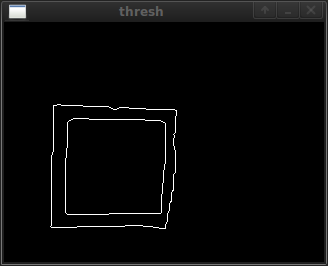
\includegraphics[scale=1.0]{figures/canny.png}
   	 \caption{Result of doing Canny edge detection on tag regions}\label{fig:canny_edge}
    \end{centering}
\end{figure}

To achieve higher certainty in finding contours a set of morphological operators was applied to the binary image to make sure that shapes really consists of a set of connected components. A single pass of a dilation mask was enough.

If a suitable region was found cut out this region of interest (hereafter referred to as ROI) and throw away the rest. Experiments show that this ROI tends to be around 60x60 pixels. 

Before explaining the next step (prepare ROI) we have to understand the reason behind it. The basic idea behind template matching is to take an image and let a another smaller image (the template) 'slide' over. The region of the original image where the template has the best match (with some degree of error) is considered the winning region. If we where to match agains several templates (which we will) we simply repeat the same procedure with each tag and the one with smallest error is considered to be the best match.

Now, given a set of predefined tags, if we where to make sure that all templates, and the possible tag we would like to match against, would have the same size it means that we could skip the step of 'sliding' one image over the other and limit ourselves to doing one matching per template to calculate the error degree for each template. The template with the smallest error is clearly the best match and the image can now be classified according to this match. Continuing this idea of same structure, when initializing the templates we convert them all to a resolution of 50x50, threshold them into binary images and make sure the border around each template is completely removed to make sure we have as simple structure as possible.

Returning to the (possible) tag in a ROI. The prepare step consist of executing this previously explained procedure. The only difference is we have to take factors such as rotation, skew, if the ROI contains borders or not, into consideration. The result is a ROI with same structure as the set of templates, namely: binary image of size 50x50 pixels.

\begin{figure}[h]
\label{fig:thresh}
    \begin{centering}
   	 
\includegraphics[scale=1.2]{figures/thresh.png}
   	 \caption{A prepared tag ROI (resized, thresholded and blurred)}\label{fig:thresh}
    \end{centering}
\end{figure}

The classification is now easy, we simply loop through and match agains each template, best match is the winner. If the error vector is to big we can't make any conclusions with enough level of certainty so we classify the tag as 'UNKNOWN'. A question the reader now should be asking themselves is: ''Would higher resolution of tags/templates give higher degree of certainty in the results?''. We tested with resolutions up to around 300x300 for the tag ROI and templates with an source image resolution of 640x480 and the answer is no. The end result was that we where able to correctly classify the same amount of tags with high resp. low input resolutions. The question is still open for even higher resolution, in which we believe the results would be better, but the tradeoff with the extreme increase in computational cost it was not considered to be worth it.

\subsection{Color Detection}
To determine the color of the now classified object. Since we know that the color of a tag would be one of four previously defined colors simply sum up the number of pixels belonging to different color categories and the one with highest sum is the resulting color class. To reduce the amount of noise and to make sure we did not take border pixels into account we sampled a small region of the center (30\% going outwards) of the tag ROI this was possible since every source tag contained colors pixels in the middle.

We found the intervals for the different color regions by empirically studying histograms of captured frames for various tag colors and it worked surprisingly well for the distinct colors of green, blue and magenta. Detecting black colors proved to be much more difficult (since black is the absence of all colors). Since every capture image contains noise and a black color vector doesn't have any magnitude we instead used a little trick: if the capture ROI consists of an even spread (the amount of pixels will be low) of colors for green, blue, magenta we conclude that the object must be black. This also worked very well and from experiments we detect the correct color in roughly 9 of 10 cases.

\begin{figure}[h]
\label{fig:histogram}
    \begin{centering}
   	 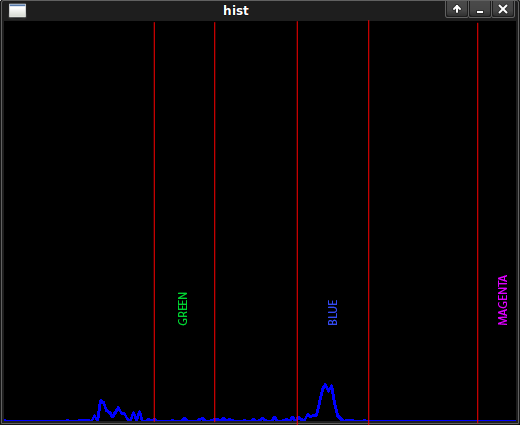
\includegraphics[scale=0.7]{figures/histogram.png}
   	 \caption{Adaptive thresholding of color regions (here a blue tag is detected)}\label{fig:histogram}
    \end{centering}
\end{figure}
